\documentclass[preprint,12pt]{elsarticle}

\usepackage[T1]{fontenc}
\usepackage{amsmath}
\usepackage{amssymb}
\usepackage{graphicx}
\usepackage{booktabs}
\usepackage{array}
\usepackage{url}
\usepackage{xcolor}
\usepackage{tabularx}
\newcolumntype{L}{>{\raggedright\arraybackslash}X}
\newcolumntype{P}[1]{>{\raggedright\arraybackslash}p{#1}}
\newcolumntype{R}[1]{>{\raggedleft\arraybackslash}p{#1}}
\def\UrlBreaks{\do\/\do-\do_}
\def\UrlBigBreaks{}
\urlstyle{same}
\setlength{\emergencystretch}{2em}
\renewcommand{\topfraction}{0.85}
\renewcommand{\bottomfraction}{0.7}
\renewcommand{\textfraction}{0.1}
\renewcommand{\floatpagefraction}{0.7}

\begin{document}

\newcommand{\anwg}{\mathrm{ANWG}}
\newcommand{\sbs}{\mathrm{SBS}}
\newcommand{\vbs}{\mathrm{VBS}}
\newcommand{\policy}[1]{\texttt{\detokenize{#1}}}

\begin{frontmatter}

\title{When Does LLM-Serving Scheduler\\
Adaptation Matter?\\
Action Opportunity and Causal Headroom\\
in Production-Derived Replay}

\author{Soroush Vahidi}

\address{New Jersey Institute of Technology, Newark, NJ, USA}

\begin{abstract}
Adaptive scheduling for large language model (LLM) serving pays off only if the system reaches states with a different executable action that improves performance. We measure that opportunity before designing any adaptive scheduler. In a deterministic simulator replaying production-derived traces (Azure code, Azure conversation, BurstGPT), we count how often six policies propose an action different from a fixed reference and, on fresh windows, force one alternative for one step before returning to it. With abundant resources, replay was action-null in about one million decision states. Capping key-value (KV) cache capacity or concurrent sequences created disagreement; scaling arrival rates up to eight times left the system lightly loaded and created none. On untouched windows this held for the Azure traces but not BurstGPT, which never queued enough for the caps to bind. In a pre-specified analysis of 720 fresh disagreement states, 590 (81.9\%) had positive latency headroom (state-weighted mean 2.00 ms; 95\% window-clustered confidence interval 0.19--3.55 ms). The sign is stable; the magnitude is not: the median is 0.20 ms, one of 36 windows holds 88\% of the total, and in 14\% of states every alternative is worse. About 95\% of the headroom lies where all five other policies differ from the reference. A bounded vLLM probe shows pressure changes scheduler behavior but does not validate the simulated latency effect. Opportunity is real but sparse, concentrated, and reference-conditional; finding it does not show that adaptive scheduling is worthwhile.
\end{abstract}

\begin{keyword}
LLM serving \sep request scheduling \sep performance evaluation \sep workload replay \sep resource contention \sep causal evaluation
\end{keyword}

\end{frontmatter}

\section{Introduction}
\label{sec:introduction}

Adaptive scheduling in large language model (LLM) serving is usually motivated
by heterogeneous prompts, decode demand, key-value (KV) cache residency,
queueing, and deadlines. It can help only if the live system reaches states
where a different executable action exists, such as another admission, batch,
or request order, and only if taking that action improves the target metric by
more than the cost of choosing it. How often this happens is not usually
reported alongside a scheduler design.

Common evaluation practice does not answer this. Ranking policies on
whole-trace metrics, or reporting the gap to a virtual best solver (VBS) as in
algorithm portfolios~\cite{rice1976algorithmselection,gomes2001portfolios},
shows that policies differ but aggregates thousands of decisions; it cannot say
whether an alternative was available at a given state. Policies with different
scores can issue the same batch, and an alternative that exists may not reduce
latency. Recent systems address \emph{how} to
adapt~\cite{llumnix2024,sola2025,distserve2024,lmetric2026}. We ask the prior
question: \emph{when is there a different useful action to take, and how much
is it worth?}

We answer it with a staged decomposition,
\begin{equation}
  \begin{aligned}
  \text{resource pressure}&\longrightarrow P(D)\longrightarrow
  P(B_{\mathrm{LAT}}\mid D)\\
  &\longrightarrow\text{headroom magnitude}\\
  &\longrightarrow\text{predictability and deployment}.
  \end{aligned}
  \label{eq:chain}
\end{equation}
Here $D$ means that at least one canonical executable alternative differs from
the default single best scheduler (SBS), a fixed reference policy described in
Section~\ref{sec:methods}, and $B_{\mathrm{LAT}}$ that at least one such
alternative lowers one-step mean latency relative to that reference. These are
distinct quantities: pressure can make policies disagree often without the
disagreement being useful, and useful disagreement can be rare or small. All of
them are conditional on the reference and the portfolio. The last arrow,
whether a selector could exploit the opportunity, is not measured here
(Figure~\ref{fig:pipeline}).

\begin{figure}[!htbp]
\centering

\includegraphics[scale=1]{figures/pe_pipeline.pdf}
\caption{Staged evidence chain (Eq.~\ref{eq:chain}): resource pressure,
canonical action disagreement $P(D)$, beneficial disagreement
$P(B_{\mathrm{LAT}}\mid D)$, headroom magnitude $H_{\mathrm{LAT}}$, and
predictability and deployability. The study measures the first four stages
(solid boxes); the fifth (dashed box) is not measured.}
\label{fig:pipeline}
\end{figure}

This is a performance-evaluation question: at which operating points does
scheduler choice have causal performance consequences? Answering it takes
workload characterization, controlled resource interventions, replay-based
simulation, and inference that respects the dependence among states from one
trace window. It complements recent work in \emph{Performance Evaluation} on
assignment, dispatching, and prediction mechanisms (Section~\ref{sec:related}).

We replay production-derived traces (Azure 2023 code and
conversation~\cite{azurepublicdataset2023}, BurstGPT~\cite{burstgpt2025}) in a
deterministic simulator. Faithful replay of 60 windows gives the native
baseline; one-axis interventions on active-sequence capacity, KV capacity, and
arrival rate (1,080 conditions) locate where disagreement appears. We repeat
that matrix on fresh non-overlapping windows and, at each disagreement state in
the selected regimes, clone the simulator, force one alternative action once,
and return to the reference. The primary endpoint, oracle latency headroom (the
largest one-step mean-latency reduction among the alternatives, zero if none
helps), was pre-specified before any outcome was computed
(Section~\ref{sec:endpoint}); the robustness analyses are post hoc. A bounded
vLLM~\cite{vllm2023} probe checks the mechanism in a real engine.

Native replay is action-null under abundant resources. Capacity caps on active
sequences or KV cache create disagreement, whereas arrival-rate scaling up to
eight times never loaded the simulated system enough to bind any resource and
creates none. On untouched windows the cap transition reproduces for the two
Azure traces but not for BurstGPT, whose windows never queued enough for the
caps to bind. Of 720 fresh disagreement states, 590 (81.9\%; 589 excluding one
floating-point-residue state) had positive headroom, with a state-weighted mean
of 2.00 ms (95\% window-clustered confidence interval 0.19--3.55 ms). The sign
survives every reweighting and leave-one-out analysis; the magnitude does not:
the median is 0.20 ms, only 22.5\% of states offer more than 2 ms, one of 36
windows carries 88\% of the total headroom, and about 95\% of it lies where all
five other policies differ from the reference. Opportunity is thus real but
sparse, concentrated, and conditional on the reference; the oracle is an
opportunity bound, not a scheduler.

The study addresses five research questions, ordered along the decomposition.
\begin{description}
\item[RQ1 -- Native opportunity.] How often does the SBS face a different
executable action from the six-policy portfolio in faithful replay with
abundant resources?
\item[RQ2 -- Pressure-induced opportunity.] Which of the tested capacity caps and
arrival rates create action disagreement, and does the transition reproduce on
untouched windows in every workload?
\item[RQ3 -- Causal value.] At disagreement states, how often does forcing one
alternative action for one step reduce latency?
\item[RQ4 -- Magnitude and concentration.] How large and how concentrated is the
headroom, and how sensitive is it to weighting, to individual windows or
regimes, and to the reference policy?
\item[RQ5 -- System correspondence.] Does a bounded vLLM probe show the
corresponding pressure and scheduling mechanism?
\end{description}

\subsection{Contributions}
This paper proposes no new scheduler. The scheduling heuristics, replay
simulation, KV-capacity constraints, and bootstrap inference it uses are
established components; the contribution is a measurement built from them and
its application.
\begin{enumerate}
  \item A staged action-opportunity evaluation that separates executable
  disagreement, beneficial disagreement, and headroom magnitude from
  policy-score diversity, with prevalence measured over all valid decision
  states, uncertainty quantified by trace window, and every quantity stated
  relative to a fixed reference scheduler.
  \item A characterization of where disagreement appears in these replays:
  capacity limits on active sequences or KV cache expose alternatives, whereas
  arrival-rate scaling up to eight times, which never loaded the simulated
  system, does not. The transition reproduces on untouched Azure windows but
  not on untouched BurstGPT windows, which never queued enough for the caps to
  bind.
  \item A pre-specified one-step causal measurement on 720 fresh states, with
  latency as the primary endpoint because deadline goodput saturates, and with
  harm structure and relative headroom reported as secondary outcomes.
  \item A robustness, concentration, and reference-dependence analysis showing
  that the sign of the headroom is robust but its magnitude is concentrated in
  one window and in states where the reference differs from all other policies.
  \item Bounded system evidence that resource pressure changes queueing and
  scheduling behavior in vLLM, without validating simulated latency magnitudes
  or a deployed selector.
\end{enumerate}

Section~\ref{sec:related} positions the work and Section~\ref{sec:methods}
defines the design, estimands, and endpoints. Sections~\ref{sec:disagreement}
to~\ref{sec:robust} report where disagreement appears, the causal headroom, and
its concentration and reference dependence; Section~\ref{sec:real} reports the
vLLM probe, and Sections~\ref{sec:discussion} and~\ref{sec:conclusion} interpret
and conclude.

\section{Related Work and Positioning}
\label{sec:related}

LLM-serving research spans model execution, prefill/decode scheduling,
resource management, routing, caching, and cluster control. Orca and vLLM
established iteration-level serving and paged KV management
\cite{orca2022,vllm2023}; Sarathi-Serve, DistServe, Splitwise, and FastServe
study chunked prefill, phase separation, and preemptive scheduling
\cite{sarathi2024,distserve2024,splitwise2024,fastserve2026}. Llumnix
reschedules requests across instances and SOLA schedules with awareness of
request and system state \cite{llumnix2024,sola2025}; Preble co-optimizes
KV-state reuse and load balancing across GPUs~\cite{preble2025}; Libra studies
flexible request partitioning \cite{libra2026}; Mooncake and Strata emphasize
KV-centric or hierarchical context caching~\cite{mooncake2025,strata2025};
MorphServe changes model precision and KV capacity under
pressure~\cite{morphserve2025}; and DynamoLLM reconfigures cluster resources for
performance and energy \cite{dynamollm2025}. BurstGPT and the Azure traces
provide workload evidence~\cite{burstgpt2025,azurepublicdataset2023}, and Nixon
et al. study workload evolution, caching, and load balancing over a year of
production traffic~\cite{yearllmserving2026}.

ServeGen characterizes and generates production LLM
workloads~\cite{servegen2025}, and OpenTela unifies decentralized computing
resources for heterogeneous LLM serving~\cite{opentela2026}. LMetric combines a
KV-aware indicator with an instance-load indicator, reports production-style
workloads, and derives conditions under which its multiplicative combination
can fail~\cite{lmetric2026}. Analytical work studies online scheduling under a
KV-cache memory limit, with competitive-ratio guarantees and a hindsight-optimal
benchmark~\cite{jaillet2025online}, and the role of service-time predictions in
queueing models of LLM scheduling~\cite{mitzenmacher2025queueing}. Simulators
such as Vidur predict latency from profiled operator costs~\cite{vidur2024};
the simulator used here is not calibrated in that way (Section~\ref{sec:methods}).
The question here precedes these works: in a fixed workload and resource regime, do a fixed
reference scheduler and its alternatives expose different executable actions at
all, and does forcing one alternative have reference-relative causal value? The
hindsight benchmark of Jaillet et al. is the closest analytical counterpart; it
compares an online algorithm with a hindsight-optimal integer program, whereas
the measurement here is empirical, one-step, and tied to the states a specific
reference visits in replay.

Recent papers in \emph{Performance Evaluation} address neighboring problems:
job assignment in machine-learning inference systems with accuracy
constraints~\cite{choudhury2025job}, dispatching policies in data-center
clusters studied on Google and Alibaba workloads~\cite{yildiz2026dispatching},
resource-aware latency prediction for GPU-accelerated model
serving~\cite{liang2026lilou}, and adaptive machine-learning training on
serverless clouds~\cite{ali2025enabling}. This paper asks whether, in a given
workload and resource state, an alternative scheduling action exists and has
causal one-step value relative to a fixed reference scheduler, before a
mechanism for choosing among actions is designed.
Table~\ref{tab:closest} summarizes the systems closest to this measurement.

\begin{table*}[tbp]
\centering
\footnotesize
\caption{Systems closest to this study, by focus and the level at which they
act, and their relation to the present measurement.}
\label{tab:closest}
\setlength{\tabcolsep}{4pt}
\renewcommand{\arraystretch}{1.15}
\begin{tabularx}{\linewidth}{@{}P{0.17\linewidth}P{0.31\linewidth}P{0.17\linewidth}L@{}}
\toprule
Work & Focus & Level & Relation to this study \\
\midrule
ServeGen~\cite{servegen2025} & Characterization and generation of production LLM workloads & Workload model & Source of workload structure; no scheduling action measured \\
LMetric, Preble~\cite{lmetric2026,preble2025} & KV-aware and load-aware request routing & Across instances & Mechanisms whose routing states this measurement could examine \\
OpenTela~\cite{opentela2026} & Orchestration of decentralized clusters for LLM serving & Across clusters & Operation of the serving fabric, not action opportunity \\
Llumnix, SOLA~\cite{llumnix2024,sola2025} & Cross-instance rescheduling; state-aware iteration scheduling & Across and within instances & Adaptive mechanisms whose opportunity this measurement targets \\
Mooncake, Strata~\cite{mooncake2025,strata2025} & KV-centric architecture and scheduling; hierarchical context caching & KV placement, scheduling & KV capacity is also a pressure axis studied here \\
Jaillet et al.~\cite{jaillet2025online} & Online scheduling under a KV-cache memory limit, with competitive-ratio analysis & Within an engine & Analytical counterpart of the KV axis; hindsight benchmark \\
This study & Existence and one-step counterfactual value of alternative actions & Within one engine, per step & --- \\
\bottomrule
\end{tabularx}
\end{table*}

The reference points of a best fixed policy and a virtual best solver come from
algorithm portfolios and selection
\cite{rice1976algorithmselection,gomes2001portfolios,satzilla2008,autofolio2015}.
Here the SBS is a fixed default whose executable actions are compared with those
of the other policies; the contribution is that application to scheduler actions
in the staged characterization of Eq.~\ref{eq:chain}, not a new selection
method.

\section{Methods}
\label{sec:methods}

\subsection{Workloads and simulator}
\label{sec:workloads}
The evidence comes from three kinds of experiment on production-derived traces.
Native replay of unmodified windows answers RQ1. One-axis transformations of
those windows (caps on active sequences or KV capacity, and arrival-rate
scaling) answer RQ2, first on the original windows, which served as the
development set for the pressure map, and again on untouched ones. A
pre-specified one-step intervention on the untouched windows answers RQ3 and
RQ4, and the vLLM probe answers RQ5.

The faithful corpus contains 20 windows of 200 requests from each of Azure 2023
code, Azure 2023 conversation, and BurstGPT, with source order and token-length
and arrival structure retained. Every replay runs on one simulated GPU (512
active-sequence slots, a 512-token batch budget, 8,000,000 KV tokens by default)
with a 1~ms step, so absolute latencies are in simulator units, not calibrated
to hardware. Each request carries a loose service-level objective (SLO) deadline
of arrival plus 1000~s, a uniform priority of 1.0, and a single class, and
policies observe a predicted output length equal to the true length. No request
therefore approaches its deadline (the largest mean continuation latency in any
causal population is 0.36~s), and deadline- and priority-sensitive rules receive
no informative signal.

A second set of 20 untouched windows per workload, taken as the first unused
contiguous windows in trace order and sharing no source records with the first,
tests whether the pressure transition reproduces and supplies the states for the
causal intervention. Those states come from five pressure regimes chosen
mechanically from the support map of the untouched windows (the onset,
sustained, and strongest valid setting on each axis that showed disagreement)
without using any latency outcome. A pressure condition is a workload window
plus one fixed one-axis intervention, such as a KV-capacity cap, active-sequence
cap, or arrival-rate scaling factor. A \emph{decision state} is one invocation
of the reference policy.

\subsection{Scheduling policies and reference}
The portfolio contains six policies implemented in the study's own simulator:
full prefill and small-chunk prefill (64-token chunks), which share one
arrival-order admission rule and differ only in execution chunk size;
estimated-service-first (ESTF), which admits the smallest estimated service time
(prompt length plus predicted output length); weighted fair sharing (WFS), which
ranks by class share and estimated service; least-laxity first (LLF), which
ranks by slack to the deadline; and the KV-constrained online policy described
below. They are simple heuristics named after standard scheduling rules, not
reimplementations of published serving systems.

All six read the same observable state: each waiting request's arrival time,
prompt length, predicted output length, deadline, priority, and class, and each
GPU's capacity and KV occupancy. Because the predicted output length equals the
true length, the service-time estimates are exact. Four policies use it (ESTF,
WFS, LLF, and the reference); the two prefill variants use only arrival order.
The rules are therefore oracle-informed heuristics rather than deployable
schedulers, and the results describe this idealized information setting. The
portfolio is also functionally less diverse than six names suggest. The two
prefill variants issue the same action from any state. With one class and
uniform priority, WFS's class-share term is constant, and in the 720 causal
states it differs from the reference in exactly the same 519 states as ESTF.
LLF ranks by slack to deadlines 1000~s away. At the 720 disagreement states the
portfolio offers on average 1.15 distinct alternative actions, and 610 states
have exactly one.

The reference (default) scheduler is the single best scheduler (SBS), the
KV-constrained online policy. It had the highest mean goodput among the six
policies on an earlier benchmark of 240 multi-mechanism scenarios from the same
project, run with the same simulator and policy implementations on scenarios
other than these trace windows. It was fixed before the fresh evaluation and is
not selected, tuned, or changed using fresh outcomes; it is best only among these
six policies on that benchmark and is not claimed to be optimal or strong here.
It was not tuned to these workloads or to latency. It orders waiting requests by
KV footprint and admits a request only if the resulting KV utilization stays at
or below a reserve of 0.82 of the configured capacity, unless the request is
urgent (slack under 0.25~s), an exemption that never applies with 1000~s
deadlines. Every measurement below is therefore relative to this reference and
its reserve. Three notions of KV pressure are kept apart: the imposed capacity
setting (the cap value); physical binding, when the waiting prompt tokens exceed
the free KV capacity (for the active-sequence cap, when no sequence slot is
free); and the reference's own reserve threshold, which can withhold admission
before capacity is physically exhausted.

\subsection{Action opportunity and one-step headroom}
Let $\mathcal{A}_6(s)$ be the set of canonical executable actions produced by
the six portfolio policies at state $s$, after action deduplication. A
canonical action is the simulator-executable admission, batch, and request
ordering decision after infeasible or semantically identical variants have
been collapsed. Let $a_{\sbs}(s)$ be the SBS action. We define
\begin{equation}
  D(s) = \mathbf{1}\left[\exists a\in\mathcal{A}_6(s):
  a\ne a_{\sbs}(s)\right].
  \label{eq:disagreement}
\end{equation}
The opportunity prevalence is $P(D)=\sum_sD(s)/|\mathcal{S}_{\mathrm{all}}|$,
where the denominator is every valid decision state, not only states where
policy scores differ. A policy ranking change that produces the same admission,
batch, and request order is action collapse, not opportunity. An alternative
action is any executable member of $\mathcal{A}_6(s)$ that is not equal to
$a_{\sbs}(s)$.

For every disagreement state $s$ and canonical alternative $a$, we clone the
state, force exactly one action, and return to the SBS for the continuation.
Let $L_{\mathrm{CF}}(s,a)$ be the mean latency of the resulting continuation and
$L_{\sbs}(s)$ that of the unmodified SBS continuation; both cover the active,
queued, and future requests of the continuation and exclude requests completed
before $s$. This is a local counterfactual, not selector performance: it
estimates the one-step effect of changing the current action while holding the
subsequent policy fixed. We define
\begin{equation}
 \begin{aligned}
 A_{\mathrm{LAT}}(s,a)&=L_{\sbs}(s)-L_{\mathrm{CF}}(s,a),\\
 H_{\mathrm{LAT}}(s)&=\max\left(0,\max_aA_{\mathrm{LAT}}(s,a)\right),
 \end{aligned}
 \label{eq:latency}
\end{equation}
where positive values reduce mean latency. The beneficial-state indicator is
$B_{\mathrm{LAT}}(s)=1$ iff $\max_aA_{\mathrm{LAT}}(s,a)>0$. We report
$P(B_{\mathrm{LAT}}\mid D)$ and mean $H_{\mathrm{LAT}}$ separately from $P(D)$,
so the conceptual aggregate opportunity is
\begin{equation}
 P(D)\times P(B_{\mathrm{LAT}}\mid D)\times
 \text{effect magnitude},
 \label{eq:decomposition}
\end{equation}
not an exact deployable-performance equation. A high conditional benefit can
coexist with a tiny overall opportunity. ``Support'' and ``opportunity'' refer
only to the existence of executable non-SBS actions under a condition;
usefulness requires the causal latency test above.

\subsection{Endpoints and pre-specification}
\label{sec:endpoint}
Deadline goodput is the natural objective for a deadline-constrained service,
and we measured it first as arrival-normalized weighted goodput (ANWG),
\begin{equation}
 \anwg = \frac{\sum_iw_i\mathbf{1}[i\text{ completes by its SLO}]}{\sum_iw_i}.
 \label{eq:anwg}
\end{equation}
An earlier causal run on the original windows found every terminal ANWG value
equal to 1.0: with deadlines 1000~s after arrival every request finished on
time, and ANWG separates met from missed deadlines but not differences in
latency or queueing, although most counterfactual branches changed latency.
Mean latency (Eq.~\ref{eq:latency}) is therefore the primary endpoint of the
fresh study, and the earlier post hoc latency analysis is not used as
confirmatory evidence.

The relative headroom $H_{\mathrm{REL}}(s)=H_{\mathrm{LAT}}(s)/L_{\sbs}(s)$ is
the oracle reduction as a share of the reference's mean latency. The other
secondary outcomes are the state structure (some alternative reduces latency,
every alternative increases it, or neither) and the shares of alternative
actions that reduce, increase, or leave latency unchanged. The specified
p95-latency effects are stored with the action-level results but are not
reported here, and ANWG was not captured in the fresh execution.

The confirmatory analysis was specified before any outcome was computed. Its
protocol (primary endpoint, regime-selection rule, causal population, cluster
unit, bootstrap settings, and decision rule) was committed to the project's
version-controlled repository on 19 September 2026, and the results were
committed 2 h 14 min later. It was not deposited in an external registry, and
the author controlled the repository, so we call the analysis pre-specified
rather than preregistered. The decision rule requires a positive state-weighted
mean headroom and a window-clustered 95\% lower endpoint above zero. One
implementation error was corrected after the outcomes were known: the first
bootstrap grouped windows by an index shared across workloads (26 clusters)
instead of the specified source window (36 clusters). The point estimate and the
decision were unchanged.

\subsection{Statistical analysis}
\label{sec:posthoc}
The confirmatory mean uses a window-clustered percentile bootstrap with 2,000
replicates and seed 20260920. The cluster unit is the fresh trace window,
identified by workload source and window index, so multiple states from one
window do not become independent experimental units. The analyses in
Section~\ref{sec:robust} were specified after the fresh outcomes were known.
They qualify the pre-specified result and do not replace it: the endpoint
$H_{\mathrm{LAT}}$, the strict criterion $B_{\mathrm{LAT}}$, the 720 states, and
the selected regimes are unchanged. A \emph{window} is a workload source and
window index (36 windows contribute states); a \emph{regime} is a workload,
pressure axis, and pressure setting pooled over windows (five selected regimes).

\emph{Practical thresholds.} For $\epsilon\in\{0.1,0.25,0.5,1,2,5\}$~ms we
report the number and share of disagreement states with
$H_{\mathrm{LAT}}(s)>\epsilon$, that is \mbox{$P(H_{\mathrm{LAT}}>\epsilon\mid D)$},
and the number of windows containing at least one such state.

\emph{Numerical residue.} The pre-specified criterion is applied unchanged in
double precision. Simulated latency differences are integer multiples of the
decode step divided by the request population, so no genuine advantage is
smaller than about $5.2\times10^{-6}$~s; only to identify floating-point
residue, we also count states whose best advantage exceeds $10^{-12}$~s.

\emph{Aggregation.} For a unit $u$ (a window, regime, or workload source) let
$D_u$ be its disagreement states and
$\bar H_u=|D_u|^{-1}\sum_{s\in D_u}H_{\mathrm{LAT}}(s)$. The pre-specified
estimate is the \emph{state-weighted mean}
$\bar H=|D|^{-1}\sum_{s\in D}H_{\mathrm{LAT}}(s)$, in which every state has
weight $1/|D|$. The \emph{equal-window}, \emph{equal-regime}, and
\emph{equal-workload} means are $U^{-1}\sum_u\bar H_u$ over the 36 windows, five
regimes, or two workloads, so every unit has weight $1/U$. These are different
estimands, not alternative estimates of one quantity; the beneficial share is
aggregated in the same way. Intervals use the same window-clustered percentile
bootstrap with 200,000 replicates; for the equal-regime and equal-workload
means, regimes and workloads are fixed strata, which ignores dependence between
regimes that share a window.

\emph{Leave-one-out, concentration, and interval diagnostics.} For each window
(36) and each regime (5) we recompute the state-weighted mean and beneficial
share from the remaining states with a window-clustered bootstrap interval
(200,000 replicates). Concentration is the share of the total summed headroom
$\sum_sH_{\mathrm{LAT}}(s)$ contributed by each window and regime, and the
effective number of windows $1/\sum_wp_w^2$, where $p_w$ is the share of window
$w$. To check the confirmatory interval we repeat the percentile bootstrap with
$10^6$ replicates and add a bias-corrected and accelerated (BCa) interval and a
delete-one-window jackknife $t$ interval; these are diagnostics, not
replacements.

\section{Where Disagreement Appears}
\label{sec:disagreement}

\subsection{Native replay}
\label{sec:native}
Under the abundant-resource baseline, all three production-derived workloads
were canonically action-null (Figure~\ref{fig:disagreement}). Azure code had 0
disagreements in 99,992 SBS decision states; Azure conversation had 0 in
461,985; and BurstGPT had 0 in 440,461. The corresponding maximum KV
utilizations were 0.0027, 0.0017, and 0.0038, with no active-cap binding states,
and the mean queue lengths were 0.040, 0.0087, and 0.0091 requests, so the
replay was lightly loaded. Policy-ranking proxy scores differed in a small
number of states, but the canonical actions collapsed to the SBS action. In this
resource regime the six-policy portfolio offered no executable alternative.

\begin{figure}[!htbp]
\centering

\includegraphics[scale=1]{figures/pe_disagreement_rates.pdf}
\caption{Disagreement prevalence $P(D)$, the percentage of SBS decision states
that are disagreement states (counts in the axis labels), for native replay of
the three workloads and for selected pressure conditions (conv. = conversation).
Native replay produced no disagreement state. Fill denotes the pressure axis.}
\label{fig:disagreement}
\end{figure}

\subsection{Capacity pressure}
\label{sec:pressure}
The pressure map of the original windows evaluated 1,080 one-axis conditions:
20 windows per workload family, each under settings on the active-sequence,
KV-capacity, and arrival-rate axes (Table~\ref{tab:transition}).
Of these, 926 conditions were valid and unconstrained, 38 partially
constrained, 96 strongly constrained, and 20 horizon-invalid. Across valid
conditions, 11,328 canonical disagreement states were observed.

Arrival scaling through $8\times$ remained action-null for all three workload
families. It also left the simulated system lightly loaded: peak KV utilization
stayed below 0.71\% of the default capacity, at most 46 sequences were active
against a limit of 512, the mean queue length per workload stayed below 0.09, and
no capacity constraint bound. Disagreement first appeared at an active-sequence
cap of 16 (BurstGPT), 8 (Azure code), or 4 (Azure conversation), and at a KV
capacity of 16,000 tokens in all three workloads (Table~\ref{tab:transition}). Disagreement became sustained, in at
least two windows, at caps of 8 (BurstGPT) and 4 (Azure code and conversation)
and at KV capacities of 16,000 (Azure code and BurstGPT) and 8,000 (Azure
conversation).

\begin{table}[!htbp]
\centering
\small
\caption{Pressure settings at which canonical disagreement first appears.
Settings are the active-sequence cap (concurrent sequences) and the KV
capacity (tokens). ``First binding'' is the first setting at which the
constraint binds; ``sustained'' is the first setting with disagreement in at
least two windows.}
\label{tab:transition}
\setlength{\tabcolsep}{5pt}
\renewcommand{\arraystretch}{1.25}
\begin{tabularx}{\linewidth}{@{}lLR{0.13\linewidth}R{0.16\linewidth}R{0.12\linewidth}@{}}
\toprule
Workload & Pressure axis & First binding & First disagreement & Sustained \\
\midrule
Azure code & Active-sequence cap & 8 & 8 & 4 \\
Azure code & KV capacity & 16,000 & 16,000 & 16,000 \\
Azure conversation & Active-sequence cap & 4 & 4 & 4 \\
Azure conversation & KV capacity & 8,000 & 16,000 & 8,000 \\
BurstGPT & Active-sequence cap & 16 & 16 & 8 \\
BurstGPT & KV capacity & 16,000 & 16,000 & 16,000 \\
\bottomrule
\end{tabularx}
\end{table}

Table~\ref{tab:transition} is the main regime result: in these replays,
disagreement appeared only after an active-sequence or KV capacity was
tightened, and the arrival-rate range tested never reached a capacity limit. For
Azure conversation under a KV cap, disagreement appears at 16,000 tokens, before
the constraint physically binds at 8,000; Section~\ref{sec:refdep} examines this
pattern.

\section{Causal Headroom on Untouched Windows}
\label{sec:fresh}

\subsection{Support on untouched windows}
The 1,080-condition pressure matrix was repeated on 60 untouched windows, 20 per
workload, before any latency outcome was computed. The transition reproduced
for both Azure traces: disagreement first appeared at a KV capacity of 16,000
tokens and at active-sequence caps of 8 (Azure code) and 4 (Azure conversation),
the onset settings of Table~\ref{tab:transition}, and arrival-rate scaling again
produced none, with peak KV utilization below 0.45\%. It did not
reproduce for BurstGPT. All 360 untouched BurstGPT conditions were valid, none
produced a disagreement state, and none had a binding capacity constraint: the
untouched windows never queued more than three requests, so even the tightest
caps (four active sequences, 8,000 KV tokens) were never reached, whereas native
replay of the original BurstGPT windows reached a queue of 31 requests. Support
therefore depends on the trace and its windows as well as on the capacity
setting. The causal intervention covers five selected Azure regimes
(active-sequence and KV-capacity caps) with 720 disagreement states in total.

\subsection{Primary result}
The confirmatory intervention found 590 beneficial
states (Table~\ref{tab:fresh}; Figure~\ref{fig:regimemap}), giving
$P(B_{\mathrm{LAT}}\mid D)=590/720=0.8194\ (81.9\%)$.
Mean oracle latency headroom was 0.001995791 s (1.9958 ms), with a clustered
95\% confidence interval (CI) of [0.000190884, 0.003546196] s
([0.1909, 3.5462] ms). The pre-specified decision rule was met. The result
establishes measurable reference-relative latency opportunity at disagreement
states, whereas whether its magnitude exceeds the engineering cost of adaptation
is a separate question. The conditional share is defined on disagreement states
only. Because $P(D)$ is below 0.5\% in every selected regime
(Table~\ref{tab:fresh}), it is not the share of all scheduler decisions that
could be improved.

These pre-specified values are state-weighted over disagreement states drawn
from 36 windows and should be read with the post hoc analyses of
Section~\ref{sec:robust}: the typical state has a much smaller headroom
(median 0.20~ms), and the mean is highly concentrated in one window. One of the
590 beneficial states has an advantage of $5.6\times10^{-17}$~s, exactly one
unit in the last place of the 0.357~s latencies compared, with both branches
completing the same requests; a post hoc guard of $10^{-12}$~s gives
589/720 (81.8\%) and changes the mean by less than $10^{-19}$~s.

\begin{table}[!htbp]
\centering
\small
\caption{Fresh causal characterization by selected regime, numbered as in
Figure~\ref{fig:regimemap} (conv. = conversation; active cap
= active-sequence cap; KV = KV capacity in tokens). $P(D)$ is the percentage of
valid SBS decision states in the regime's conditions that are disagreement
states, $P(B_{\mathrm{LAT}}\mid D)$ the percentage with positive oracle headroom,
and mean $H_{\mathrm{LAT}}$ the state-weighted mean. Windows can contribute to
several regimes, so window counts are not additive; the 36 distinct
workload--window pairs are the bootstrap clusters.}
\label{tab:fresh}
\footnotesize
\setlength{\tabcolsep}{4pt}
\renewcommand{\arraystretch}{1.2}
\begin{tabularx}{\linewidth}{@{}LR{0.075\linewidth}R{0.11\linewidth}R{0.085\linewidth}R{0.145\linewidth}R{0.095\linewidth}R{0.12\linewidth}@{}}
\toprule
Regime & States & Windows & $P(D)$ (\%) & $P(B_{\mathrm{LAT}}\mid D)$ (\%) & Mean $H_{\mathrm{LAT}}$ (ms) & Headroom share (\%) \\
\midrule
(1) Azure code,\newline active cap 8 & 10 & 2 & 0.0106 & 40.0 & 0.033 & 0.02 \\
(2) Azure code,\newline active cap 4 & 122 & 15 & 0.129 & 52.5 & 0.077 & 0.65 \\
(3) Azure code,\newline KV 16,000 & 431 & 14 & 0.456 & 92.3 & 3.227 & 96.80 \\
(4) Azure conv.,\newline active cap 4 & 64 & 17 & 0.0108 & 48.4 & 0.217 & 0.97 \\
(5) Azure conv.,\newline KV 16,000 & 93 & 1 & 0.0157 & 100.0 & 0.241 & 1.56 \\
\midrule
All selected regimes & 720 & 36 & --- & 81.9 & 1.996 & 100.00 \\
\bottomrule
\end{tabularx}
\end{table}

\begin{figure}[!htbp]
\centering

\includegraphics[scale=1]{figures/pe_regime_map.pdf}
\caption{Regime map for the five selected regimes, numbered as in
Table~\ref{tab:fresh}. Horizontal axis: disagreement prevalence $P(D)$ in
percent (logarithmic scale). Vertical axis: beneficial share
$P(B_{\mathrm{LAT}}\mid D)$, which counts any positive headroom (regime 5, at
100\%, has a mean headroom of 0.24~ms). Marker area is proportional to the mean
oracle headroom; fill denotes the pressure axis.}
\label{fig:regimemap}
\end{figure}

Figure~\ref{fig:regimemap} separates prevalence from value. Azure-code KV
capacity = 16,000 has the largest selected $P(D)$ and the largest mean headroom;
active-cap regimes have much smaller $P(D)$ and correspondingly smaller
aggregate opportunity even when some states are beneficial. All three factors
of Eq.~\ref{eq:decomposition} therefore need measuring: whether a different
action exists, whether it helps conditional on existing, and whether its effect
is large enough to matter against noise and control overhead.

\subsection{Secondary outcomes}
\label{sec:secondary}
Table~\ref{tab:secondary} reports the pre-specified secondary outcomes.
Disagreement is not automatically opportunity, even in sign: in 102 of the 720
states (14.2\%) every alternative increases latency, and 141 of the 831
alternative actions (17.0\%) do so. The median relative headroom is 0.21\%, but
92 states (12.8\%) exceed 10\% of the reference's mean latency, and all 92 lie in
the Azure-code KV-capacity = 16,000 regime, where they are 21.3\% of the states.

\begin{table}[!htbp]
\centering
\small
\caption{Pre-specified secondary outcomes over the 720 fresh disagreement states
and their 831 alternative actions. Relative headroom is
$H_{\mathrm{LAT}}(s)/L_{\sbs}(s)$, the oracle latency reduction as a share of the
reference's mean latency in the state. ``Zero headroom'' states have no
beneficial alternative but not every alternative harmful.}
\label{tab:secondary}
\setlength{\tabcolsep}{6pt}
\renewcommand{\arraystretch}{1.2}
\begin{tabularx}{\linewidth}{@{}Lr@{}}
\toprule
Outcome & Result \\
\midrule
\multicolumn{2}{@{}l@{}}{\emph{State structure (720 states)}} \\
Some alternative reduces latency & 590 (81.9\%) \\
\quad of which some alternative also increases it & 22 \\
Every alternative increases latency & 102 (14.2\%) \\
Zero headroom, not every alternative harmful & 28 (3.9\%) \\
\midrule
\multicolumn{2}{@{}l@{}}{\emph{Action level (831 alternative actions)}} \\
Reduce latency & 660 (79.4\%) \\
Increase latency & 141 (17.0\%) \\
Leave latency unchanged & 30 (3.6\%) \\
\midrule
\multicolumn{2}{@{}l@{}}{\emph{Relative headroom $H_{\mathrm{REL}}$}} \\
Median & 0.21\% \\
90th percentile & 11.3\% \\
90th percentile, Azure-code KV 16,000 only & 16.1\% \\
States above 1\% & 211 (29.3\%) \\
States above 5\% & 133 (18.5\%) \\
States above 10\% & 92 (12.8\%) \\
\bottomrule
\end{tabularx}
\end{table}

\section{Concentration, Sensitivity, and Reference Dependence}
\label{sec:robust}

The pre-specified result of Section~\ref{sec:fresh} is a state-weighted mean
over 720 disagreement states drawn from 36 windows. This section asks, post hoc,
how large the headroom is in a typical state, how far the mean depends on which
windows and regimes contribute (Section~\ref{sec:posthoc}), and how it depends
on the reference policy; the pre-specified criterion and estimate are not
modified.

\subsection{Effect scale and distribution}
Table~\ref{tab:thresholds} counts the states whose headroom exceeds each
practical threshold. The 81.9\% beneficial share is not the share of states
that offer material gains: 60.0\% of states exceed 0.1~ms, 29.4\% exceed 0.5~ms, 22.5\%
exceed 2~ms, and 17.9\% exceed 5~ms. The larger effects are also concentrated.
Above 0.5~ms, 201 of the 212 states belong to the Azure-code KV-capacity = 16,000
regime, and only 4 of the 36 windows contain a state above 2~ms.

\begin{table}[!htbp]
\centering
\small
\caption{Post hoc practical-effect thresholds: disagreement states whose oracle
headroom $H_{\mathrm{LAT}}$ exceeds each threshold. The first row is the
pre-specified criterion; the second excludes one floating-point-residue state
with a $10^{-12}$~s guard. ``Windows'' counts the windows (of 36) with at least
one such state; ``In KV 16,000'' counts states from the Azure-code
KV-capacity = 16,000 regime, which contributes 431 of the 720 states.}
\label{tab:thresholds}
\setlength{\tabcolsep}{5pt}
\renewcommand{\arraystretch}{1.15}
\begin{tabular}{@{}lrrrr@{}}
\toprule
Criterion & States & Share & Windows & In KV 16,000 \\
\midrule
Pre-specified ($>0$, strict) & 590 & 81.9\% & 32 & 398 \\
Guarded ($>10^{-12}$~s) & 589 & 81.8\% & 32 & 398 \\
\midrule
$>0.1$~ms & 432 & 60.0\% & 17 & 327 \\
$>0.25$~ms & 322 & 44.7\% & 16 & 259 \\
$>0.5$~ms & 212 & 29.4\% & 9 & 201 \\
$>1$~ms & 188 & 26.1\% & 7 & 185 \\
$>2$~ms & 162 & 22.5\% & 4 & 161 \\
$>5$~ms & 129 & 17.9\% & 2 & 128 \\
\bottomrule
\end{tabular}
\end{table}

The distribution is strongly right-skewed (Figure~\ref{fig:robust}a). The
median headroom is 0.197~ms, about one tenth of the 1.996~ms state-weighted mean,
and 77.4\% of states lie at or below that mean. The 90th and 95th percentiles are 8.4 and 11.3~ms, and the maximum is 12.1~ms. A further 130 states (18.1\%) have exactly zero headroom. Among the
589 states with positive headroom the median is 0.29~ms.

\begin{figure}[!htbp]
\centering
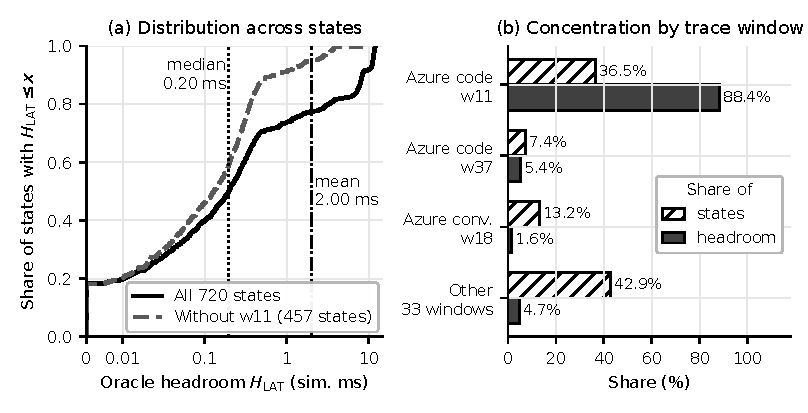
\includegraphics[scale=1]{figures/pe_robustness.pdf}
\caption{Distribution and concentration of oracle headroom over the 720
disagreement states. (a) Empirical distribution of $H_{\mathrm{LAT}}$ with and
without Azure-code window w11; zero headroom is the intercept at $x=0$, and the
axis is linear below 0.01~ms and logarithmic above. Dotted and dash-dotted lines
mark the median and the state-weighted mean. (b) Share of the 720 states
(hatched) and of the total headroom (solid) for the three largest windows and the
remaining 33.}
\label{fig:robust}
\end{figure}

\subsection{Sensitivity to aggregation and to individual windows and regimes}
Every aggregation of Table~\ref{tab:sensitivity} yields a positive mean whose
interval excludes zero, but the magnitude depends on what is weighted: from
1.996~ms (state-weighted) to 0.327~ms (equal-window), a factor of about six, and
the beneficial share falls from 0.819 to 0.632. The state-weighted mean is the
pre-specified estimand and answers ``what is the expected headroom at a
disagreement state drawn from this sample''; the equal-window and equal-regime
means answer the same question for a typical window or regime and are not
interchangeable with it.

Leaving one unit out gives the same picture. All 36 single-window and 5
single-regime omissions leave a positive mean, and every corresponding
bootstrap interval excludes zero. Omitting Azure-code window w11 leaves 0.365~ms
(95\% CI [0.158, 0.682]~ms); omitting the Azure-code KV-capacity = 16,000 regime leaves
0.159~ms (95\% CI [0.058, 0.234]~ms). Omitting any other window changes the mean only to between
2.00 and 2.26~ms, and omitting any other regime to between 2.02 and 2.39~ms.
The sign therefore survives all 41 omissions, whereas the headline magnitude
does not survive the omission of the two dominant units.

\begin{table}[!htbp]
\centering
\small
\caption{Post hoc sensitivity of the mean oracle headroom to the aggregation rule and
to leaving out the two dominant units. Each unit has equal weight except in the
state-weighted row, where each state does. ``Share'' is the beneficial share
under the strict $>0$ criterion. The state-weighted interval is the
confirmatory one (2,000 replicates); the others are window-clustered
percentile bootstrap intervals with 200,000 replicates (Section~\ref{sec:posthoc}).}
\label{tab:sensitivity}
\setlength{\tabcolsep}{4pt}
\renewcommand{\arraystretch}{1.15}
\begin{tabular}{@{}llccc@{}}
\toprule
Estimand & Units & Mean (ms) & 95\% CI (ms) & Share \\
\midrule
State-weighted (pre-specified) & 720 states & 1.996 & [0.191, 3.546] & 0.819 \\
Equal-workload & 2 workloads & 1.360 & [0.184, 2.094] & 0.809 \\
Equal-regime & 5 regimes & 0.759 & [0.145, 1.161] & 0.666 \\
Equal-window & 36 windows & 0.327 & [0.114, 0.644] & 0.632 \\
\midrule
\multicolumn{5}{@{}l}{\emph{Leave one out: state-weighted mean of the remaining states}} \\
Omit Azure-code window w11 & 457 states & 0.365 & [0.158, 0.682] & 0.821 \\
Omit Azure-code KV 16,000 & 289 states & 0.159 & [0.058, 0.234] & 0.664 \\
\bottomrule
\end{tabular}
\end{table}

\subsection{Concentration of headroom}
Window w11 of the Azure-code trace contains 263 of the 720 states (36.5\%) but
contributes 88.4\% of the total summed headroom; the three largest windows
contribute 95.3\%, and the effective number of windows by headroom mass is
1.27 (5.7 by state count). At regime level, Azure-code KV-capacity = 16,000
holds 59.9\% of the states and 96.8\% of the headroom, contributing 1.93 of
the 2.00~ms state-weighted mean. Within w11, 205 states of that regime average
6.16~ms. Of the 129 states above 5~ms, 128 are in w11, as are 140 of the 162
states above 2~ms (Figure~\ref{fig:robust}b). The state-weighted mean is thus
highly concentrated in a narrow high-headroom subset of states and should not
be read as the typical benefit of a disagreement state. Appendix~A shows that the width of
the confirmatory interval reflects this concentration, not simulation noise.

\subsection{Dependence on the reference scheduler}
\label{sec:refdep}
The SBS is a fixed heuristic, and the headroom is measured against it. In 512 of
the 720 disagreement states (71\%) all five other policies differ from the SBS,
and these states carry 94.8\% of the total headroom; 511 of them lie in the two
KV-capacity regimes, and in 445 the five policies agree on a single alternative
action. The disagreement is therefore mainly between the reference and the rest
of the portfolio, not among the alternatives. The KV-capacity regimes contain 524
disagreement states, of which 414 occur without physical KV binding (the waiting
prompt tokens fit in the free capacity) and hold 89.6\% of those regimes'
headroom. These are valid observations: the reference reorders or withholds
admissions there although capacity is not exhausted. Physical exhaustion
therefore does not explain them. The reference's 0.82 reserve and its
KV-footprint ordering, which no other portfolio policy uses, are the candidate
sources, and this analysis does not separate the two. The headroom is best read
as room for improving on this reference under a capped KV capacity, not as a
general property of KV-limited serving.

\section{A Bounded vLLM System Correspondence Probe}
\label{sec:real}

The probe used one RTX 5060 Ti GPU, vLLM 0.27.1, Qwen2.5-0.5B-Instruct, and
deterministic token-shape replay. It comprised 40 full-versus-chunked runs and
a 20-run native chunked-prefill budget probe, with queueing and scheduler
traces retained. It separates three levels of evidence. Level 1, one-step
headroom at disagreement states, is established only in the controlled replay.
Level 2, that resource pressure changes observable queueing and scheduling
behavior, is supported in vLLM. Level 3, that a deployed adaptive selector
would recover the simulated headroom or improve end-to-end latency, SLOs, or
throughput, is not established.

The native budget probe held chunked prefill fixed and varied the per-step
token budget (512 tokens, T512, versus 4,096 tokens, T4096). T512 produced
1,680 scheduler steps, 165 mixed prefill/decode steps, and 194 partial-prefill
items; T4096 produced 1,536, 55, and 9. Waiting queues reached lengths of 7 and
5, respectively, while running sequences reached 4 in both cases. The low-load
regime showed a 30.6~ms difference in late time to first token and a 16.3~ms
prompt-heavy end-to-end tradeoff; the high-load regime showed a smaller
time-to-first-token difference and a 23.3~ms prompt-heavy end-to-end tradeoff.

The direct full-versus-chunked comparison did not reproduce the simulator's
qualitative reversal. KV-utilization and preemption
metrics could not be collected in the native probe. The probe therefore shows that concrete serving pressure
alters observable scheduling behavior and latency; it does not estimate
Eq.~\ref{eq:latency} in the real system.

The simulator's one-step, reference-relative effect has no vLLM counterpart,
because an exact one-step intervention is not available in the engine.

\section{Discussion}
\label{sec:discussion}

\subsection{Sign and magnitude of the headroom}
The fresh study establishes that positive one-step headroom exists: under the
pre-specified criterion, forcing an alternative action lowers mean latency in
590 of 720 disagreement states (81.9\%), and the sign is stable across the
aggregation and omission analyses of Section~\ref{sec:robust}. The magnitude is
not. The state-weighted mean of 2.00~ms (95\% window-clustered CI
[0.19, 3.55]~ms) estimates the expected headroom at a state drawn from this
sample, not the headroom of a typical state: the median is 0.20~ms, and the mean
falls to 0.33~ms when windows receive equal weight
(Table~\ref{tab:sensitivity}). ``Beneficial'' is a criterion on the sign of the
causal effect, not on its operational size: 22.5\% of disagreement states offer
more than 2~ms, in 14.2\% every alternative is worse than the reference, and
relative to the reference's latency the median headroom is 0.21\% while 12.8\%
of states exceed 10\%, all in one regime (Table~\ref{tab:secondary}). One
Azure-code window carries 88.4\% of the total headroom, the Azure-code
KV-capacity = 16,000 regime carries 96.8\%, and the effective number of windows
by headroom mass is 1.27 (Figure~\ref{fig:robust}). An aggregate mean can
therefore conceal highly localized scheduling opportunity, so the distribution
of effects, the prevalence of material effects, and the sensitivity to
aggregation belong next to any overall mean. The same concentration explains the
width of the confirmatory interval, which remains the inference of record
(Appendix~A).

\subsection{Opportunity, prediction, and deployment}
Adaptive scheduling should be evaluated in stages, because each stage can fail
while the previous one holds. Resource pressure need not produce executable
disagreement: native replay encountered no alternative action in about one
million decision states. Disagreement need not be beneficial, a positive effect
need not be material, and a material oracle effect need not be recoverable. The
estimand is one-step oracle headroom under SBS continuation: one alternative
action is forced at a disagreement state, and the default then resumes.
$H_{\mathrm{LAT}}(s)$ selects the best alternative after the outcomes are
observed, so it answers whether a useful action existed at $s$, not whether an
online system could have identified it, and it does not measure a selector,
longer-horizon switching, or adaptation overhead.

Each stage is also measured against one fixed reference and one portfolio. About
95\% of the headroom lies where all five other policies differ from the
reference, and most KV-regime disagreement occurs without physical KV binding
(Section~\ref{sec:refdep}), so the measurement is largely the room to improve on
this reference's reserve and ordering under a capped KV capacity, not evidence
that the portfolio is complementary. Score-level complementarity is a separate
question: on the 60 native windows, small-chunk prefill has a higher whole-window
mean latency than full prefill in all 60 (median 14.2\%), yet the two issue the
same action from any state and differ only in execution chunk size, so no
per-state choice can realize that gap. The data illustrate the possibility
without measuring a six-policy gap, which was not evaluated in the faithful
view.

\subsection{Resource pressure and action support}
Caps on active sequences and KV capacity created disagreement in all three
workloads on the original windows (Section~\ref{sec:disagreement}), whereas
arrival-rate scaling up to eight times left every workload action-null. This is
a negative result under light load: the simulated GPU never approached a
capacity limit (peak KV utilization below 1\% of the default capacity), so it
does not show that arrival intensity cannot create opportunity in a congested
system. It shows that, in these production-derived workloads under controlled
resource interventions, disagreement appeared only after a capacity setting was
tightened, and where a trace enters that regime depends on its windows: BurstGPT
disagreement appeared in the original windows but not in the untouched ones, so
the onset settings of Table~\ref{tab:transition} are not workload constants. The
vLLM experiment is a bounded system correspondence probe
(Section~\ref{sec:real}): it shows that pressure changes queueing and scheduling
behavior in a real engine, did not reproduce the simulator's qualitative
reversal in the direct full-versus-chunked comparison, and does not validate the
simulated headroom magnitude or an adaptive-scheduler gain.

\subsection{Implications for practice}
The evidence supports a measurement-first practice, not a scheduler
recommendation.
\begin{itemize}
  \item Measure executable action disagreement before building a selector;
  diversity in policy scores is not evidence of it.
  \item Characterize which resource constraints bind, in addition to the arrival
  rate, and state the reference policy and how it was chosen.
  \item Report the distribution of effects in absolute and relative terms, their
  concentration, and the share of states in which every alternative is harmful,
  alongside any oracle mean.
  \item Weigh the recoverable gain against selector, monitoring, and switching
  costs; the median disagreement state offers only 0.20~ms, and outside the few
  regimes with material opportunity a fixed scheduler may be the appropriate
  policy.
\end{itemize}
The study demonstrates no production savings, deployed-selector benefit, or
capacity-planning gain.

\subsection{Limitations and threats to validity}
The limitations below bound what the evidence supports.
\begin{description}
  \item[Policy portfolio.] The six policies are simple heuristics, two sharing
  an admission rule and two reducing to one ranking under the overlays, and four
  using exact output lengths. They do not span modern production serving
  systems, and other portfolios may expose different action support.
  \item[Reference scheduler.] The SBS is a fixed heuristic chosen on an earlier
  benchmark, with a hard-coded 0.82 KV reserve that the measured headroom partly
  reflects (Section~\ref{sec:refdep}). Conclusions are conditional on it, and a
  differently tuned reference could shrink or shift the opportunity.
  \item[Workload overlays.] Deadlines are 1000~s after arrival, priority and
  class are constant, and predicted output lengths equal true lengths, so
  deadline- and priority-sensitive rules receive no informative signal,
  length-aware rules face no prediction error, and goodput saturates.
  \item[Workloads.] Native replay and pressure mapping cover three
  production-derived families, but the fresh causal study covers Azure code and
  conversation only, because the untouched BurstGPT windows never queued enough
  for the caps to bind. Fresh windows were taken in trace order, not sampled at
  random.
  \item[Controlled interventions.] Active-sequence and KV caps are experimental
  interventions, not observed production provisioning, and arrival-rate scaling
  up to eight times left the simulated system lightly loaded, so the arrival
  results do not bound the effect of higher congestion.
  \item[One-step oracle.] $H_{\mathrm{LAT}}$ isolates one-step causal
  opportunity with an ex post best alternative; it is not closed-loop
  adaptation.
  \item[Concentration.] The magnitude rests on few windows, with an effective
  number of about 1.27 by headroom mass. The sign has broader support: 32 of the
  36 windows contain a state with positive headroom.
  \item[System correspondence.] The probe uses one model, one GPU, one vLLM
  version, token-shape replay, and incomplete instrumentation, so it supports
  only the qualitative mechanism.
  \item[Objective.] Mean latency is the primary causal endpoint; the goodput
  saturation shows that the objective changes the measured opportunity
  (Section~\ref{sec:endpoint}), and tail-latency and SLO-violation objectives
  were not evaluated.
  \item[External validity.] Other models, hardware, schedulers, and
  context-length distributions may show a different opportunity structure, and
  absolute milliseconds are simulator units. The staged protocol transfers; the
  measured magnitudes need not.
\end{description}

\section{Conclusion}
\label{sec:conclusion}

This paper asked whether an LLM-serving scheduler ever faces an executable alternative worth taking. Replay of production-derived traces under abundant resources offered none: in about one million decision states, no policy proposed an action different from the single best scheduler (SBS), a fixed reference. Capacity caps on active sequences or KV cache created such states, whereas arrival-rate scaling up to eight times left the system lightly loaded and did not. On the Azure traces, forcing an alternative once lowered latency in most of these states (590 of 720 under the pre-specified criterion).

The opportunity is small, concentrated, and conditional. The state-weighted mean of 2.00~ms is not a typical effect: the median disagreement state offers 0.20~ms, the mean falls to 0.33~ms when windows are weighted equally, and one trace window holds 88.4\% of the total. Most of the headroom lies where the reference alone differs from the rest of the portfolio, so it measures room to improve on that reference.

The lesson for performance evaluation is to establish, stage by stage, that executable disagreement, causal benefit, and a material effect exist before adding selector complexity, and to report the reference, the portfolio, the load range, and the distribution of effects with any measured opportunity. Adaptation is justified by where the measured opportunity lies, not by its average.

\section*{Appendix A. Interval Diagnostics}
Monte Carlo error does not explain the width of the confirmatory interval.
With $10^6$ replicates the percentile interval is [0.184, 3.543]~ms, no
replicate has a nonpositive mean, and the lower endpoint of the 2,000-replicate
procedure varies by only 0.004~ms (standard deviation) across 1000 seeds. The BCa
interval is [0.239, 4.049]~ms. The bootstrap distribution is bimodal: 36\% of
replicates do not draw window w11 and have a mean of about 0.36~ms, against
2.43~ms for those that do, so the percentile interval spans the gap between
two populations of replicates. The delete-one-window jackknife $t$ interval,
[$-1.36$, 5.35]~ms, includes zero because one influential window inflates its
standard error (1.65~ms); all 36 delete-one estimates are positive, and we
treat the jackknife interval as a diagnostic of this dependence rather than as
a competing interval. Uncertainty about the magnitude of the headroom thus
reflects its concentration in few windows, not simulation noise.

\section*{Declaration of generative AI and AI-assisted technologies in the manuscript preparation process}
During the preparation of this work, the author used ChatGPT (OpenAI), Codex (OpenAI), Gemini (Google), and Claude (Anthropic) in order to assist with organization, language editing, literature-search planning, and drafting analysis, figure, and test code. After using these tools, the author reviewed and edited the content as needed and takes full responsibility for the content of the publication.

\section*{Declaration of Competing Interest}
The author declares that they have no known competing financial interests or personal relationships that could have appeared to influence the work reported in this paper.

\section*{Acknowledgements}
The author gratefully acknowledges Professor Ioannis Koutis for research guidance and scientific feedback. The author thanks the NJIT Wulver HPC for providing computational resources for the fresh confirmatory computation, and Anders Borum (Secure ShellFish) for providing tools that enabled remote research access. Finally, the author thanks his mother for her continued support.

\section*{Funding and Support}
This work received in-kind computational support through the Google Cloud Research Credits Program (USD 1,000 in cloud credits) and computational/tooling support from CloudRift Inc. Neither Google nor CloudRift Inc. had any role in the study design, data collection, analysis, interpretation, manuscript preparation decisions, or the decision to submit the article for publication. No monetary research grant was received from these organizations.

\section*{Data and Code Availability}
{\leavevmode\raggedright Code, derived research artifacts, experiment configurations, and reproducibility materials for this study are available in the GitHub repository \url{https://github.com/SoroushVahidi/llm-serving-heuristic-evolution} (release \texttt{performance-evaluation-v1.1.0}) and are permanently archived on Zenodo \cite{vahidi2026archive}. The archive is a snapshot of that release: the published v1.0.0 record predates the post hoc robustness analysis, and the materials it lacks (the robustness outputs, the corrected derivative, the continuation shards, the figure code, and the claim manifest) are available in the GitHub repository only until the v1.1.0 version of the archive is published. The v1.1.0 archive contains the frozen confirmatory artifacts (native replay, pressure mapping, and fresh causal latency headroom), the post hoc robustness outputs (Section~\ref{sec:robust}), a corrected derivative of two descriptive state-level columns that leaves the original frozen file unchanged, the continuation shards from which that derivative is computed, the simulator and analysis code, the figure and table scripts, and the claim manifest that checks the quoted numbers. Raw third-party workload traces are not redistributed and are obtained from their original upstream sources.\par}

\bibliographystyle{elsarticle-num}

{\raggedright
\bibliography{references}
}

\end{document}
